\documentclass[11pt,a4paper]{article}

\usepackage[margin=1in]{geometry}
\usepackage{amsmath,amssymb}
\usepackage{booktabs}
\usepackage{graphicx}
\usepackage{tikz}
\usetikzlibrary{shapes,arrows,positioning}
\usepackage{hyperref}
\hypersetup{colorlinks=true,linkcolor=blue,citecolor=blue,urlcolor=blue}
\usepackage{enumitem}
\usepackage{caption}

\title{MedMNIST Pre-Warm-Up:\\Multi-Seed Reproducibility Study and Joint-Learning Proposal}
\author{Habib Ur Rehman}
\date{October 2026}

\begin{document}
\maketitle

\begin{abstract}
This report documents the pre-warm-up exercise on the MedMNIST v2 benchmark:
replicating published results with the authors' official code, quantifying
run-to-run variability across fixed random seeds, and proposing a method for
training one model jointly across datasets. A feasibility constraint forced a
documented protocol change for the 2D suite (native $28 \times 28$ ResNet-18
instead of $224 \times 224$ ResNet-50); the completed batch-1 runs
(breast, retina, pneumonia $\times$ 5 seeds) show seed spreads above 2.5
percentage points on every dataset, supporting the reproducibility concern
that motivates the study. All configurations, run records, and results are preserved
in a public working repository.\footnote{\url{https://github.com/habib-analyst/MedMNIST_v2_Reproducibility_Benchmark}}
\end{abstract}

\section{Introduction and Protocol}

The exercise follows the MedMNIST v2 publication~\cite{medmnistv2} and runs the
code released by the authors at \url{https://github.com/MedMNIST/experiments},
pinned to commit \texttt{70b6b3a}. No new model code was written for the
replication steps; the work consisted of running the official training script,
fixing random seeds, and verifying the outputs independently.

\noindent\textbf{Fixed protocol elements (all runs):}
\begin{itemize}[nosep]
    \item Optimizer: Adam, learning rate $10^{-3}$; scheduler MultiStepLR with
    milestones at epochs 50 and 75, $\gamma = 0.1$.
    \item Epochs: 100. Batch size: 128.
    \item Seeds: 17, 29, 43, 71, 101 (five per dataset).
    \item Checkpointing with automatic resume; per-run JSON logs recording
    configuration hash, metrics, and provenance.
\end{itemize}

\section{Step (a): ChestMNIST with ResNet-50 at $224 \times 224$}

The specified configuration (ResNet-50, $224 \times 224$ RGB) was attempted
first. A single 100-epoch ChestMNIST run was extrapolated at approximately
37 GPU-hours on a Kaggle T4 from measured per-epoch times, which exceeds the
available free-tier quota
($\sim$30 GPU-hours/week) for even one complete run. Two partial records exist
(a 27-epoch and a 32-epoch single-seed run, preserved under
\texttt{kaggle/evidence/} and labeled partial/exploratory). \textbf{No
complete 100-epoch ResNet-50 run has been finished; step (a) is therefore
reported as incomplete, not as a result.} This measurement is itself evidence:
the specified 2D suite ($\sim$1,150--1,200 T4 GPU-hours) is not executable
without dedicated compute, which motivated the documented protocol change
below.

\section{Step (b): Multi-Dataset Replication}

\subsection{Protocol change (documented 2026-10-07)}

Because the specified configuration is infeasible on available compute, the
multi-seed study was moved to the authors' native $28 \times 28$ ResNet-18
configuration (upstream defaults: \texttt{--size 28}, no resize,
\texttt{--model\_flag resnet18}), keeping the identical optimizer, schedule,
epochs, and seed set. This is the configuration of the published MedMNIST
leaderboard, so comparison against published reference values remains the
most apples-to-apples literature comparison available. The original
$224 \times 224$ ResNet-50 run matrix is retained in the repository as the
historical record and can be re-run if larger compute becomes available.

\subsection{Batch 1 results (2D, complete and verified)}

Fifteen of fifteen runs completed with exit code 0; metrics were
reconstructed from the run scripts' stdout logs after the Kaggle session
ended, with provenance documented in the repository
(Table~\ref{tab:batch1}).

\begin{table}[h]
\centering
\caption{Batch 1: native $28 \times 28$ ResNet-18, 100 epochs, 5 seeds per dataset.
\textit{Spread} is max$-$min test AUC across the five seeds; std is the
population standard deviation across seeds.
Published AUC values are the ResNet-50 ($224 \times 224$) reference column;
architectures differ, so the comparison is a sanity signal, not a replication claim.}
\label{tab:batch1}
\begin{tabular}{lcccc}
\toprule
Dataset & $n$ & Test AUC (mean $\pm$ std) & Spread & Published AUC (ref.) \\
\midrule
BreastMNIST    & 5 & $0.9074 \pm 0.0103$ & 0.0295 & 0.866 \\
PneumoniaMNIST & 5 & $0.9464 \pm 0.0106$ & 0.0272 & 0.962 \\
RetinaMNIST    & 5 & $0.7290 \pm 0.0081$ & 0.0255 & 0.716 \\
\bottomrule
\end{tabular}
\end{table}

The central finding of batch 1 is \textbf{seed instability}: the spread across
five fixed seeds exceeds 2.5 percentage points on every dataset, with standard
deviations around 1 point. Single-seed reported numbers therefore understate
the uncertainty of the benchmark, which is precisely the reproducibility
concern the protocol was designed to test.

\subsection{3D suite (in progress)}

Five of thirty 3D runs were executed (AdrenalMNIST3D $\times$ 5
seeds, 3D ResNet-50, 100 epochs each); per-run metric records are being
finalized in the repository. A sixth run is stalled mid-training with its
checkpoint preserved; the remaining runs ($\sim$90 GPU-hours) are blocked on
compute availability.

\section{Comparison with Reported Performance}

Table~\ref{tab:batch1} places the batch-1 means beside the published reference
AUCs. Two caveats are stated explicitly: (1) the reference column is
ResNet-50 at $224 \times 224$ while batch 1 is ResNet-18 at $28 \times 28$,
so differences confound architecture, resolution, and seed noise; (2) with
only three of twelve 2D datasets complete, no claim is made about the
benchmark as a whole. The honest summary is that batch-1 AUCs land in the same
range as the published values while exhibiting the seed variability that
single-run reporting hides.

\section{Step (c): Joint Learning Across Datasets}

\subsection{Challenges}

\begin{enumerate}[nosep]
    \item \textbf{Heterogeneous label spaces.} The 18 datasets mix binary,
    multi-class, ordinal-regression, and multi-label tasks with incompatible
    class indices; a single output layer is meaningless.
    \item \textbf{Scale imbalance.} Dataset sizes range from a few hundred to
    over 100\,000 images. Naive joint training lets the largest datasets
    dominate the gradient.
    \item \textbf{Modality gaps.} X-ray, histology, dermoscopy, OCT, retinal
    fundus, ultrasound, abdominal CT, and electron microscopy volumes share
    little low-level statistics; a single representation may suffer negative
    transfer.
    \item \textbf{Dimensionality split.} 2D and 3D inputs need different
    encoder geometries, yet the goal includes one model over all 18 datasets.
\end{enumerate}

\subsection{How to overcome them}

The design follows the accrue-and-reuse principle demonstrated in the lab's
own foundation-model work~\cite{arkplus,ark}: keep one shared representation,
preserve each dataset's native supervision with dataset-specific heads, and
control exposure so no dataset dominates. Concretely: (i) per-dataset
classification heads with the native label space and the loss appropriate to
each task; (ii) size-balanced sampling (square-root or temperature-weighted)
so small datasets are seen often enough to matter; (iii) a shared 2D encoder
for the twelve 2D datasets and a shared 3D encoder for the six 3D datasets,
with a lightweight 2.5D adapter (slice encoder plus aggregation) bridging the
two for the all-18 model; (iv) cyclic or sequential exposure of datasets with
an exponential-moving-average teacher so knowledge accrued from one dataset
persists while training on the next.

\subsection{The idea: What, Why, How, So What}

\begin{description}[nosep]
    \item[What.] A shared-encoder, multi-head architecture trained jointly:
    one model over the 12 2D datasets, one over the 6 3D datasets, and one
    unified model over all 18 via the 2D/3D adapter (Figure~\ref{fig:joint}).
    \item[Why.] Small MedMNIST datasets (e.g.\ BreastMNIST, RetinaMNIST) cannot
    support strong representations alone; shared training lets them borrow
    statistical strength, while the multi-seed study above shows single-task
    numbers are noisy enough that joint regularization may also stabilize
    them.
    \item[How.] Dataset-specific heads with native losses; temperature-weighted
    sampling across datasets; shared encoder updated by all tasks; cyclic
    dataset exposure with EMA teacher accrual; per-dataset validation tracked
    separately so negative transfer is detected, not averaged away.
    \item[So What.] If the joint model matches or beats single-dataset
    baselines with lower seed variance, it becomes a stronger, cheaper
    starting point for biomedical image classification than 18 separate
    models, and the protocol in Sections 2--4 gives the honest baseline to
    prove it.
\end{description}

\begin{figure}[h]
\centering
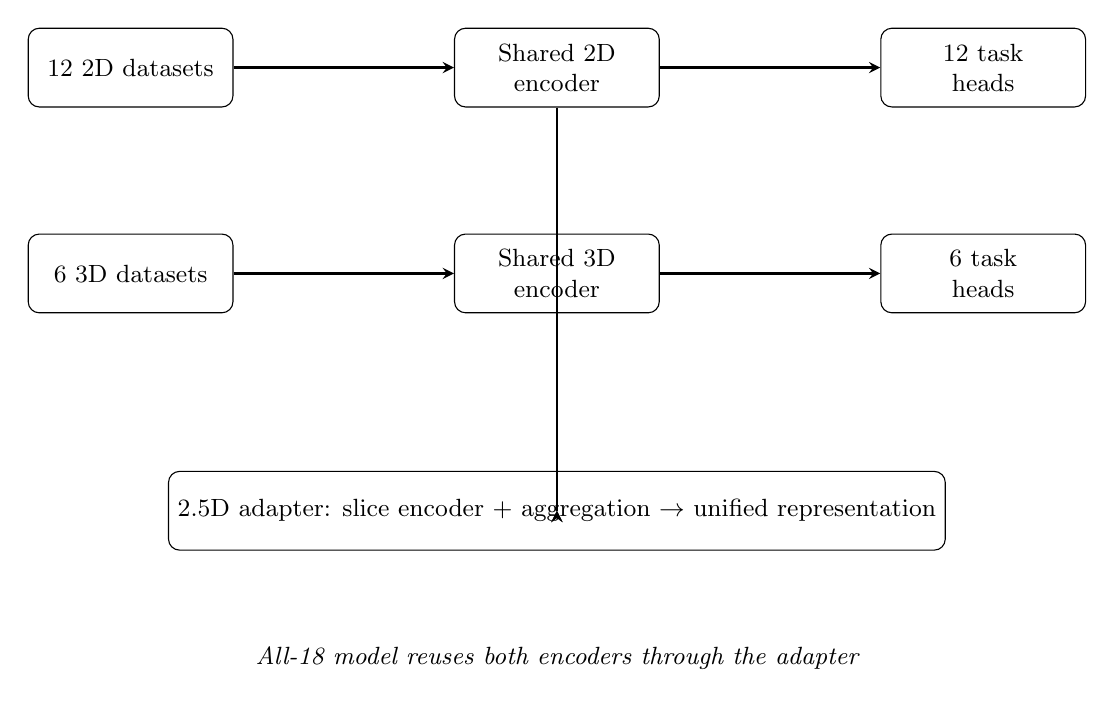
\begin{tikzpicture}[
    node distance=1.6cm, auto,
    block/.style={rectangle, draw, rounded corners, minimum width=2.6cm, minimum height=1cm, align=center, font=\small},
    arrow/.style={->, >=stealth, thick}
]
    \node[block] (d2d) {12 2D datasets};
    \node[block, below=of d2d] (d3d) {6 3D datasets};
    \node[block, right=of d2d, xshift=1.2cm] (enc2d) {Shared 2D\\encoder};
    \node[block, right=of d3d, xshift=1.2cm] (enc3d) {Shared 3D\\encoder};
    \node[block, right=of enc2d, xshift=1.2cm] (heads2d) {12 task\\heads};
    \node[block, right=of enc3d, xshift=1.2cm] (heads3d) {6 task\\heads};
    \node[block, below=of enc3d, yshift=-0.4cm, minimum width=5.5cm] (adapter)
        {2.5D adapter: slice encoder + aggregation $\rightarrow$ unified representation};
    \draw[arrow] (d2d) -- (enc2d);
    \draw[arrow] (d3d) -- (enc3d);
    \draw[arrow] (enc2d) -- (heads2d);
    \draw[arrow] (enc3d) -- (heads3d);
    \draw[arrow] (enc2d) |- (adapter);
    \draw[arrow] (enc3d) |- (adapter);
    \node[below=of adapter, yshift=0.5cm, font=\small\itshape] {All-18 model reuses both encoders through the adapter};
\end{tikzpicture}
\caption{Joint-learning design: shared encoders with dataset-specific heads;
the all-18 model bridges 2D and 3D through a 2.5D adapter.}
\label{fig:joint}
\end{figure}

\section{Limitations and Next Steps}

\begin{itemize}[nosep]
    \item Step (a) has no complete runs; the $224 \times 224$ ResNet-50 arm
    awaits dedicated compute.
    \item Nine of twelve 2D datasets and twenty-five of thirty 3D runs remain;
    the 3D suite needs roughly 90 additional GPU-hours.
    \item The joint-learning idea in Section~5 is a proposal supported by
    literature review, not an implemented or evaluated model; negative
    results from early architecture ablations are recorded in the repository
    rather than hidden.
    \item Next: finish the 2D suite on available compute, secure compute for
    the 3D suite, then implement the Section~5 design starting with the
    twelve 2D datasets.
\end{itemize}

\begin{thebibliography}{9}
\bibitem{medmnistv2}
J.~Yang, R.~Shi, D.~Wei, Z.~Liu, L.~Zhao, B.~Ke, H.~Pfister, and B.~Ni.
MedMNIST v2: A large-scale lightweight benchmark for 2D and 3D biomedical
image classification. \textit{Scientific Data}, 10:41, 2023.

\bibitem{arkplus}
D.~Ma, J.~Pang, M.~B.~Gotway, and J.~Liang. A fully open AI foundation model
applied to chest radiography. \textit{Nature}, 643:488--498, 2025.

\bibitem{ark}
D.~Ma, J.~Pang, M.~B.~Gotway, and J.~Liang. Foundation Ark: Accruing and
reusing knowledge for superior and robust performance. In \textit{MICCAI},
pages 651--662, 2023.
\end{thebibliography}

\end{document}
